% !TEX root = 00_thesis.tex

\chapter{Introduction}
\label{ch:introduction}

\TODO{
\begin{itemize}
	\item Fig4: left-align. remove white boxes
\end{itemize}
}


Cyber-Physical Systems (\CPS) are understood as systems where ``\emph{physical and software components are deeply intertwined, each operating on different spatial and temporal scales, exhibiting multiple and distinct behavioral modalities, and interacting with each other in a myriad of ways that change with context}''~\cite{nsf2010Cyber}.
The domains of application of \CPS are very diverse: \eg robotics, distributed monitoring, process control, power-grid management~\cite{stankovic2008WSAN, lee2008Cyber, rajkumar2010CPS}.

It is important to realize that the design of \CPS encompasses three main aspects, mapping to as many research fields, with their own purpose and goals: %\linebreak
% \begin{itemize}
	% \inlineitem
	The \emph{embedded hardware design} aims to extend the amount of computational resources available (\eg processing power, memory, sensors and actuators) while limiting the cost, form factor, and energy consumption of a device.
	% \linebreak
	% \inlineitem
	The \emph{communication}, either wired or wireless, aims to transmit messages between distributed devices efficiently; that is, quickly and using little energy.
	% \linebreak
	% \inlineitem
	Finally, the \emph{distributed system design} realizes the implementation of the \CPS functions, such as \eg remote monitoring and control of distributed processes.
% \end{itemize}

The goal of the overall design is to reliably provide the specified \CPS functions.
Achieving this goal relies on hardware and communication; however reaching ``perfect'' communication, such as 100\% packet reception rate, is not a goal in itself; it is merely a mean to an end. What truly matters is to fulfill the system functionality.
Typically, \CPS design aims to provide end-to-end performance guarantees, such as meeting hard deadlines between the execution of distributed tasks; for example, between the start of a sensing task to the end of the corresponding actuation tasks -- \cref{fig:e2ePerf}.
Meeting such deadlines is called \emph{providing real-time guarantees}.

\begin{figure}
  \centering
  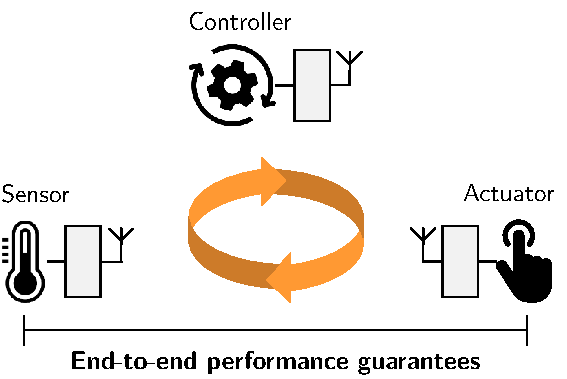
\includegraphics[scale=1]{e2ePerformance}
  \caption{The primer objective of \CPS design is to provide end-to-end performance guarantees for distributed applications.
	{In this dissertation, we consider synchronous transmissions, a recent development in low-power wireless communication, and attempt to leverage the technique to provide real-time guarantees in wireless \CPS.}}
  \label{fig:e2ePerf}
\end{figure}

The potential benefits of wireless communication for \CPS applications are well-known and include \eg simpler deployment and maintenance, cheaper operational costs, lighter weight~\cite{luvisotto2017Ultra}.
Furthermore, wireless is the only viable option in application domains including highly mobile nodes, such as an automated warehouse with transport robots~\cite{haegele2018Logistics} or teams of drones~\cite{mottola2014Teamlevela}.
However, \CPS applications have challenging performance requirements~\cite{akerberg2011Future}, which are hard to fulfill with a wireless design.


\section{Requirements of Wireless \CPS}

\CPS applications are subject to different types of requirements, such as the specified end-to-end latency, bandwidth, or number of devices; the precise performance level for these requirements depends on the application context.
Generally, \CPS requirements belong to one of the following classes:

\begin{features}[labelwidth=65pt, leftmargin=(\labelwidth+\labelsep)]

  \item[Reliability]
  A large ratio of messages are successfully transmitted wirelessly.

  \item[Adaptability]
  The system adapts to runtime changes in resource demands.

	\item[Mobility]
  The system supports mobile devices.

	\item[Timeliness]
  Applications meet their deadlines, which are often specified end-to-end. Depending on the class of systems, deadlines can be either soft or hard~\cite{buttazzo2011HardRT}.

  \item[Efficiency]
  The system
  supports short end-to-end latency,
  scales in terms of system size,
  and
  optimizes its energy consumption and bandwidth utilization.

\end{features}

These requirements are mutually conflicting. For example, reducing the energy consumption is typically achieved by keeping the radio turned off whenever possible.
However, this directly conflicts with \feature{Adaptability}, as the system cannot adapt reliably without exchanging some extra messages.
In general, there is a price to pay in terms of \feature{Efficiency} for meeting any of the other requirements.
Hence, designing \CPS consists in exploring the design space for relevant trade-offs; that is, the design optimizes the overall system \feature{Efficiency} while meeting other application requirements.



\section{Traditional Wireless Networking}
\label{sec:traditionalNetworking}

Low-power wireless communication is a mature field of research, heavily studied for more than two decades.
A large part of the research focused on wireless sensor networks, where low power consumption is a key requirement to enable long-term operation of the deployed networks, with specifications up to multiple years of operation on small batteries.
Many successful applications and deployments include monitoring of soils~\cite{geissdoerfer2019PREAct}, permafrost~\cite{weber2019decade}, buildings~\cite{chintalapudi2006Monitoring}, or wildlife~\cite{cassens2019Bursting, zhang2004Zebranet}.

In these scenarios, the distributed application often remains simple (\eg collect sensor readings).
The main challenge is to reliably aggregate or disseminate messages across a multi-hop network.
\emph{Single-hop} communication refers to the case where a source node is in communication range from its destination. This is a rather simple case, but the deployed networks often span large areas whereas low-power radios can typically communicate in the range of tens of meters.
Thus, \emph{multi-hop} communication is required, whereby a source node must rely on other nodes in the network to forward its messages, hop after hop, until the destination is reached.%
%
% \footnote
{This is the same principle as in the children's game known as Chinese whispers~\cite{ChineseWhispers}; if you ever played, you know that the original message hardly ever reaches the end of the chain successfully.}
%

Multi-hop communication is a collaborative task for which the nodes must be coordinated.
Indeed, if a node transmits a message while another wireless communication is ongoing, the transmissions will interfere and they may both fail.
% This is a key difference between wired and wireless communication: In a wired network, when a packet arrives at a switch or a router for forwarding, it can be en-queued and transmitted later; With wireless communication, packets are lost and must be retransmitted.
Furthermore, the radio frequency bands used for wireless communication cannot be isolated. Other networks are potentially exchanging messages on the same frequencies, which generates external interference and triggers packet losses.
As a result, traditional multi-hop communication requires complex mechanisms for coordinating the nodes, scheduling the different transmissions to forward all messages throughout the network, and retransmitting messages that have been lost (\eg due to external interference).
The complexity is further increased in mobile scenarios, where the set of neighboring nodes (which may relay a node's messages) changes frequently.
%
The traditional wireless networking approach performs multi-hop communication by carefully planning a sequence of unicasts (\ie one-hop transmissions), usually performed along one or a few of the shortest paths possible between a message source and its destination~\cite{watteyne2016Industrial,kim2017Challenging, mottola2011MUSTER}.
Intuitively, this is efficient because only the necessary nodes are involved in relaying a message.

In practice however, multi-hop wireless network are sensitive to topology changes, external interference, and traffic congestion. These limit the reliability of communication, which has been a major obstacle to the utilization of wireless technology in \CPS: for a long time, it has been considered impossible to provide the required level of reliability using wireless~\cite{stankovic2005Opportunities}.
Synchronous transmissions have fundamentally changed that.

\section{Synchronous Transmissions}
\label{sec:ST}

Synchronous transmissions (\ST), also referred to as concurrent transmissions, is a technique consisting in letting  multiple nodes transmit a message at the ``same time'' (hence the name of \emph{synchronous} transmissions).
A destination node can successfully receive (one of these) synchronous transmissions thanks to two effects taking place at the physical layer: constructive interference and the capture effect~\cite{yuan2013LetTalkTogether, escobar-molero2019Improving}.
In a nutshell, \ST is likely to be successful if the incoming messages arrive at the receiving node's antenna within a small time offset (in the range of a few symbol periods -- a few tens of \us~-- depending on the physical layer and the effect considered).
\ST has been shown to work both analytically~\cite{wilhelm2014Reception}, empirically~\cite{ferrari2011Glossy}, and on different physical layers, such as IEEE 802.15.4\cite{yuan2014Sparkle}, Bluetooth~\cite{alnahas2019BlueFlood}, and LoRa~\cite{wegmann2018Reliable}.

The use of \ST in low-power communication, pioneered by Glossy~\cite{ferrari2011Glossy} in 2011, has triggered a paradigm shift in the low-power wireless community: \ST can be leveraged to implement efficient broadcast in a multi-hop network using network-wide flooding~(\cref{fig:flooding}).
The flooding procedure implemented by Glossy is illustrated in \cref{fig:glossy}. A first node initiates the flooding process. The 1-hop neighbors of the initiator receive the message and synchronously broadcast this same message in the next time step, which is then received by the initiator's 2-hop neighbors with high probability, thanks to \ST. The process repeats following the same logic: a node that receives a packet broadcasts it again in the next time slot. Each node in the network transmits each packet up to $N$ times, after which the flood terminates.
It has been shown in a wide range of scenario that, with $N=3$, Glossy achieves a reliability above 99.99\%~\cite{ferrari2011Glossy}; that is, 99.9\% of the floods are successfully received by nodes in the network. With $N=5$, the average reliability reaches 99,999\%~\cite{ferrari2011Glossy}.
Glossy achieves such high reliability by leveraging spatio-temporal redundancy.
Packets are transmitted along all possible paths; in other words, they are implicitly routed everywhere, and therefore avoid interference sources localized in space.
In addition, having each node transmitting $N$ times creates temporal redundancy, thereby avoiding interference sources localized in time.
Moreover, the predictability of the operation timing in \ST-based flooding can be leveraged to perform distributed time synchronization. Glossy demonstrated that sub-\us synchronization accuracy can be achieved in a multi-hop network composed of tens to hundreds of nodes~\cite{ferrari2011Glossy}.
Since Glossy, other flooding strategies have been proposed~\cite{lim2017Competition, baddeley2019AtomicSDN, ma2019DeCoT}, but the overall principle remains the same.

\begin{figure}
  \centering
	\captionsetup[subfigure]{labelformat=empty,justification=centering}
  \begin{subfigure}[t]{0.3\linewidth}
      \centering
      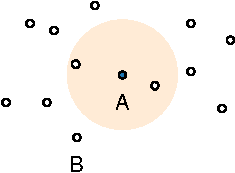
\includegraphics[scale=1]{flood_1}
			\caption{Node \textbf{A} initiates the flood.}
      \label{fig:flooding1}
  \end{subfigure}%
  \hfill
  \begin{subfigure}[t]{0.33\linewidth}
      \centering
      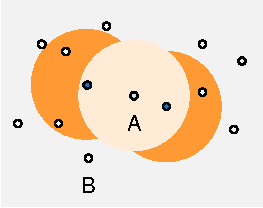
\includegraphics[scale=1]{flood_2}
			\caption{The 1-hop neighbors of \textbf{A} synchronously repeat.}
      \label{fig:flooding2}
  \end{subfigure}%
  \hfill
  \begin{subfigure}[t]{0.33\linewidth}
      \centering
      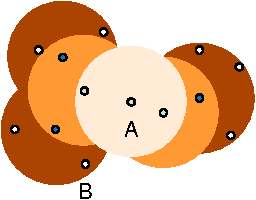
\includegraphics[scale=1]{flood_3}
			\caption{Node \textbf{B} receives the message.}
      \label{fig:flooding3}
  \end{subfigure}
  \caption{%
  Flooding process for a message sent from node \textbf{A} to node \textbf{B}}
  \label{fig:flooding}
\end{figure}

\begin{figure}
  \centering
  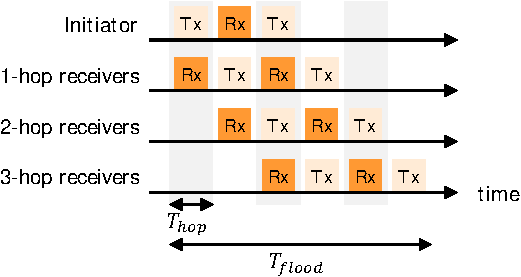
\includegraphics[scale=1]{glossy}
  \caption{Glossy operation in a 3-hop network with 2 transmissions per node ($N$)}
  \label{fig:glossy}
	\vspace{-0.2cm}
\end{figure}


The key benefit of \ST is that, thanks to the provided multi-hop broadcast primitive, the overall communication design can be dramatically simplified.
Essentially, one can abstract the underlying multi-hop topology as a \emph{virtual single-hop network}, which can scheduled like a shared bus: any node can send a message to any other node(s) in the network in bounded time. The only requirement is that no other node is using the ``bus'' at the same time.
This design, first proposed with the Low-power Wireless Bus protocol~\cite{ferrari2012LWB}, has been adapted into many different flavors~(\eg \cite{istomin2018Interferenceresilient, alnahas2017a2, sarkar2016Sleeping, baddeley2019AtomicSDN}) with always a similar concept~(\cref{fig:rounds}): communication is organized in rounds, between which nodes keep their radio turned off to save energy. Each round is composed of time slots, which are assigned to certain nodes for communication. In each of these slots, nodes execute a flooding primitive (\eg Glossy) thereby preforming a one-to-all communication.
Consequently, the complexity of performing reliable multi-hop communication (described in \cref{sec:traditionalNetworking}) is significantly relaxed.
Thanks to \ST, multi-hop communication is reduced to the scheduling of a single shared resource, a well-understood and relatively easy problem~\cite{buttazzo2011HardRT}.

\begin{figure}
  \centering
  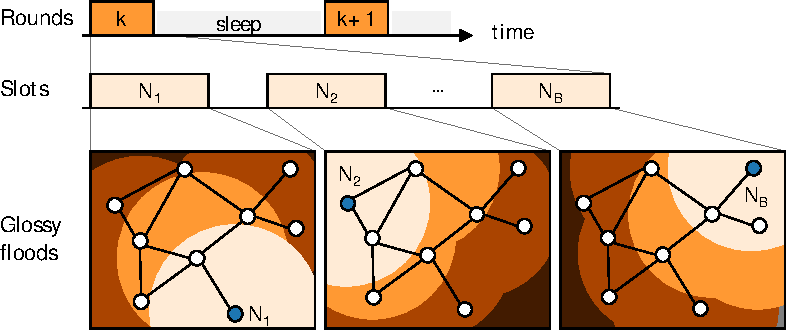
\includegraphics[scale=1]{rounds}
  \caption{Thanks to synchronous-transmissions based flooding, a multi-hop network can be abstracted and scheduled like a shared bus.
	Communication is organized in rounds, composed of time slots; in each time slot, a node initiates a flood which allows to send a message to any other node(s) in bounded time.\linebreak
	This mimics the operation of classical field bus, but with a wireless design.}
  \label{fig:rounds}
	\vspace{-0.5cm}
\end{figure}

A priori, flooding seems to be a wasteful approach: every message sent by any node will be received and forwarded by every other node in the network.
However, the simplicity and reliability of the approach actually pays off.
\linebreak
% \inlineitem
(i)~Since~the flooding logic is simple, it requires little communication overhead for the coordination of the network; nodes mostly send application data.
% \linebreak
% \inlineitem
(ii)~The~spatio-temporal redundancy embedded in the flooding process makes it very reliable; once a flood is completed, there is hardly ever a need to further retransmit a message in a subsequent flood.
% \linebreak
% \inlineitem
(iii)~Finally, since multiple nodes can transmit simultaneously, the flooding process completes quickly; very close to the theoretically optimal speed~\cite{ferrari2011Glossy}.

Thus, with flooding approaches based on \ST, the energy cost of sending one byte of data is relatively high (since this byte will be retransmitted by all the nodes), but the \emph{overall cost} for communication remains relatively small, thanks to the limited protocol overhead and the absence of need for further retransmissions.
The energy efficiency and reliability of \ST-based flooding has been demonstrated in many research contributions~(\eg \cite{ferrari2011Glossy, landsiedel2013Chaos, herrmann2018Mixer}) and showcased in the EWSN Dependability Competitions~\cite{schuss2017Competition}, where all wining solutions in the past four years (2016 to 2019) were based on \ST~\cite{escobar2018Competition, sommer2016Competition,lim2017Competition, escobar2019RedNodeBus, ma2019DeCoT}.


The downside of \ST is that it is difficult to use in more complex system designs, such as those envisioned for wireless \CPS~\cite{akerberg2011Future}.
The difficulty stems from the tight timing requirements for successful \ST: to be received reliably, transmissions must be initiated by the different nodes within few \us.
Practically, this implies that the runtime execution of a node is governed by the communication protocol, which makes the implementation of advanced distributed tasks complex and error prone.
As a consequence, \ST has thus far been mainly used for academic endeavors and mostly in wireless sensor network scenarios where the application tasks are typically simple and non-critical.
Collecting a new sensor reading is a task that can usually tolerate being delayed by a few milliseconds while communication is ongoing.\linebreak
This is generally not acceptable for wireless \CPS.

% ------------------------------------------------------------------------------
\section{The Dual-Processor Platform}
\label{sec:dpp}

In \CPS, each device must perform application and communication tasks in order to fulfill the overall system functions; this poses the challenge of interference between tasks which contend for processor execution time.
This interference problem can be mitigated by a new breed of embedded platforms featuring multiple processing cores, such as the NXP LPC541XX~\cite{nxpLPC541XX} or the VF3xxR~\cite{nxpVF3xxR}.
On the one hand, this helps because applications and communication tasks can be processed in parallel, but on the other hand, it creates contention for the access to the resources shared between the cores.
Efficient scheduling of multi-core platforms is a complex problem and a research field of its own.


Instead of resolving contention by scheduling, another approach proposed in the literature attempts to \emph{prevent interference by design}. This principle, soberly called the Dual-Processor Platform~(\DPP~-- \cite{beutel2019DPPdemo}), consists in linking two processors with a processor interconnect called \bolt~(\cref{fig:dpp}).
\bolt~\cite{sutton2015Bolt} provides predictable asynchronous message passing between two arbitrary processors while decoupling these processors with respect to time, power, and clock domains.
The lower part of \cref{fig:dpp} shows a conceptual view of the \DPP, including two message queues with first-in-first-out (FIFO) semantics, one for each direction, which are the only communication channels between the interconnected processors.
The guiding principle of \bolt design is to limit the interference between the interconnected processors as much as possible, then to provide formally verified bounds on the unavoidable interference remaining.
Concretely, this means that the \bolt API functions, used by the processors to exchange messages, have hard latency bounds.
The upper part of \cref{fig:dpp} shows an early prototype of a \DPP.
\cref{append:dpp} illustrates other \DPP designs, integrating the concept into smaller form factors and using different processors and targeting different application scenarios.



\begin{figure}
  \centering
  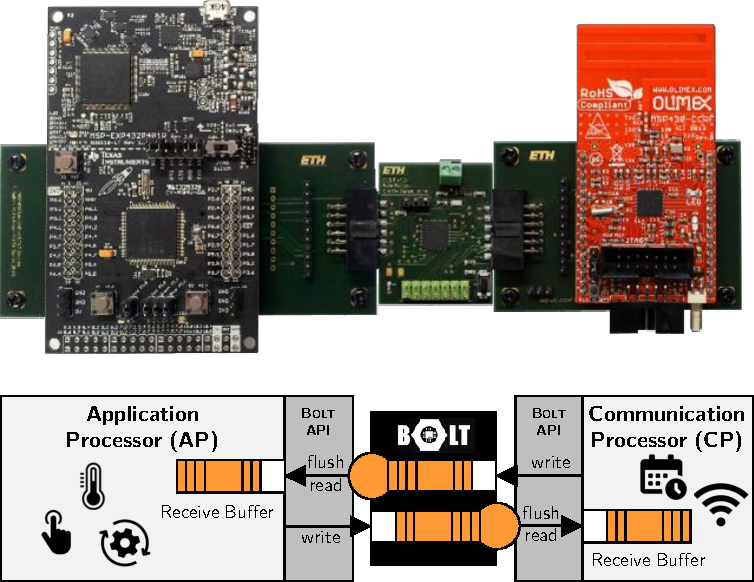
\includegraphics[scale=1]{dpp_with_pic}
  \caption{
    Top: Example of a custom-built heterogeneous \DPP.
		\capt{\bolt (in the middle) interconnects a powerful application processor (TI MSP432~\cite{msp432}) on the left with a state-of-the-art communication processor (TI CC430~\cite{CC430F6137}) on the right.}\linebreak
		%
		Bottom: Conceptual view of the \bolt processor interconnect.
		\capt{Using the \bolt's API functions (\opwrite, \opread, and \opflush), the processors dedicated to application (\AP) and communication (\CP) can asynchronously exchange messages with predictable latency, while otherwise executing independently from one another.}}
  \label{fig:dpp}
\end{figure}


The \DPP concept provides a predictable architecture for wireless \CPS nodes.
By entirely dedicating one processor to the application tasks and another one to wireless communication, we can decouple the timing of communication from the timing of the applications, and therefore facilitate the integration of \ST in a \CPS design.
Furthermore, this helps optimizing performance: each processor can be customized for the specific operations it has to perform. The division of labor fosters specialization, thereby reducing the overall energy consumption and execution time; \ie maximizing \feature{Efficiency}.

% ------------------------------------------------------------------------------
\section{Performance Evaluation in Networking}

Over the past decade, low-power wireless communication has made significant progress, which are not limited to \ST.
The overall level of performance has increased, and it is now common to see reports of packet reception rates above 99\%~\cite{ferrari2011Glossy, duquennoy2015Orchestra, duquennoy2017FiveNines, istomin2018Interferenceresilient}.

The more extreme the performance level, the more critical it becomes to confidently assess the performance.
Higher levels of confidence become necessary to argue about the differences in protocol design and quantify their performance trade-offs.
Obviously, this is import for science as it allow to compare competing approaches.
But it is also important for industry: these new and promising technologies will never be adopted unless we can back our performance claims confidently.
In other words, others must be able to reproduce our experiments.

In the context of wireless networking, reproducible performance evaluation is made particularly challenging by the inherent variability of the experimental conditions: the uncontrollable dynamics of real-world networks~\cite{matos18reproducible, burchfield09rfjungle} and the unsteady performance of hardware and software components~\cite{maricq2018Taming, blackburn2016Truth} can cause a large variability in the experimental conditions, which makes it hard to quantitatively compare different solutions~\cite{bajpai18dagstuhl_report}.

This reproducibility challenge (sometimes even referred to a ``crisis''\cite{baker16reproducibility}) touches all scientific fields, and recently received significant attention in computer science~\cite{collberg15reproducibility, saucez2018Thoughts, bajpai19dagstuhl_guide}.
Yet, how to practically design and execute performance evaluation experiments for wireless protocols remains a largely open question which is being debated by the community~\cite{boano2018IoTBench}.
The lack of a standard for evaluating performance prevents a clear comparison of the different approaches, and therefore hinders the adoption of the technology.

If everyone claims to be the best, it is difficult to trust anyone.

%%%%%%%%%%%%%%%%%%%%%%%%%%%%%%
\pagebreak
\section{Thesis Outline and Contributions}
%%%%%%%%%%%%%%%%%%%%%%%%%%%%%%

In this dissertation, we attempt to leverage recent advances in the domain of low-power wireless communication, in particular synchronous transmissions, in order to design wireless \CPS providing end-to-end real-time guarantees.
\cref{fig:chapter_all} provides an overview of the contributions of the dissertation, which are summarized below.
\begin{itemize}

  \item
  We work towards more rigorous and reproducible experimental networking research.
  For the first time, we go beyond simple guidelines and propose a concrete methodology for designing networking experiments and analyzing their data.
  We leverage this methodology to propose the first formalized definition of reproducibility for networking experiments.
  We implemented our methodology in a framework called \triscale, a first-of-its-kind tool that assists researchers by streamlining the design process and automating the data analysis~(\cref{ch:triscale}).

  \item
  We propose and implement \baloo, a design framework for network stacks based on synchronous transmissions (\ST).
  \baloo significantly lowers the entry barrier for harnessing the efficiency, reliability and mobility support of \ST:
  users implement their protocol through a simple yet flexible API while \baloo handles all the complex low-level operations based on the users' inputs~(\cref{ch:baloo}).

  \item
  We demonstrate for the first time that end-to-end real-time guarantees can be obtained in wireless \CPS by leveraging the efficiency and reliability of synchronous transmissions.
  We propose and implement wireless real-time protocols for two different design objectives.
  \begin{itemize}
    \item The Distributed Real-time Protocol (\DRP) uses contracts to maximize the flexibility of execution between application tasks~(\cref{ch:drp}).
    \item Time-Triggered Wireless (\TTW) statically co-schedules all task executions and message transfers to minimize end-to-end latency~(\cref{ch:ttw}).
  \end{itemize}

\end{itemize}


\begin{figure}[!h]
  \centering
  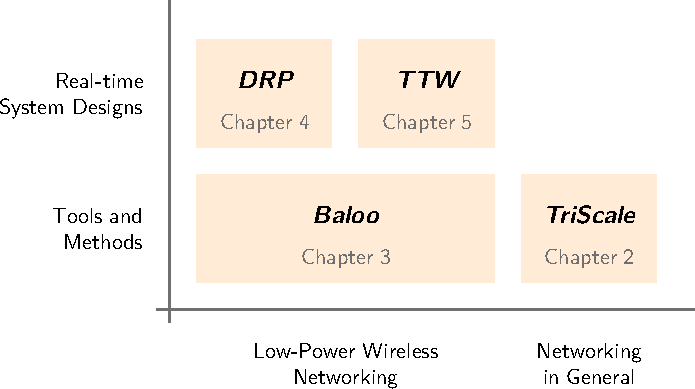
\includegraphics[scale=1]{chapter_all}
  \caption{Overview of the chapters and contributions of this dissertation.}
  \label{fig:chapter_all}
\end{figure}

% ------------------------------------------------------------------------------
% Chapter appendices
\begin{subappendices}
% ------------------------------------------------------------------------------

% ------------------------------------------------------------------------------
\newpage
\section{``Reproducible'' Dissertation}

As discussed above, one of the contribution of this dissertation attempts to foster reproducible experimental practices in networking research~(\cref{ch:triscale}).
In line with this idea, we take a step forward in that direction and attempt to make this entire dissertation ``reproducible''.

\begin{itemize}

	\item
	Each chapter includes an ``Artifacts and Links'' appendix. As the name suggests, the reader will find there various links to supplementary materials related to the corresponding chapter.

	\item
	In particular, whenever possible, we make publicly available all the data presented in this dissertation, in both raw and processed form.
	We often provide links to digital notebooks, which allow data visualization in a web browser without requiring any file download.

	\item
	All the plots in this dissertation are ``clickable''; that is, the plots are hyperlinks pointing to dynamic visualizations which let the reader explore the data (\eg zooming-in and -out in the plot, toggle visibility of individual traces, \etc).
	If you are reading a printed version of this document, you can find the corresponding link addresses in the ``Artifacts and Links'' appendices.

	\item
	The source files of this dissertation (this document) are themselves publicly available.
	\tex source files and figures are published on GitHub under the Creative Commons \href{https://creativecommons.org/licenses/by/4.0/}{CC-BY-4.0 license}.

\end{itemize}

% Finally, we must never forget that research is a collaborative endeavor.
% The work presented in this dissertation has been realized with the help of numerous colleagues and dedicated Master students, and we believe it is important to transparently credit each person for their respective contributions.
%
% We do this by using CRediT (Contributor Roles Taxonomy)~\cite{credit}, a standardized taxonomy developed and supported by CASRAI.
% CRediT is high-level taxonomy including 14 roles capturing the typical contributions to scientific scholarly outputs.
% For each chapter, we publish a so-called ``Authors Contributions Statement'' which lists the people that have contributed to the work and their respective role(s).
% These statements are available together with the dissertation files.

% ------------------------------------------------------------------------------
\newpage
\section{Dual-Processor Platforms}
\label{append:dpp}

This appendix illustrates various \DPP designs developed by the Computer Engineering Group at ETH Zurich.
These research prototypes implement the \DPP concepts described in \cref{sec:dpp}, using different processors and targeting different application scenarios. Some of these designs are used in the real-world data collection deployments reported \eg in~\cite{weber2019decade,meyer2019IPSN}.

\vspace{1cm}

\begin{figure}[h]
	\centering
	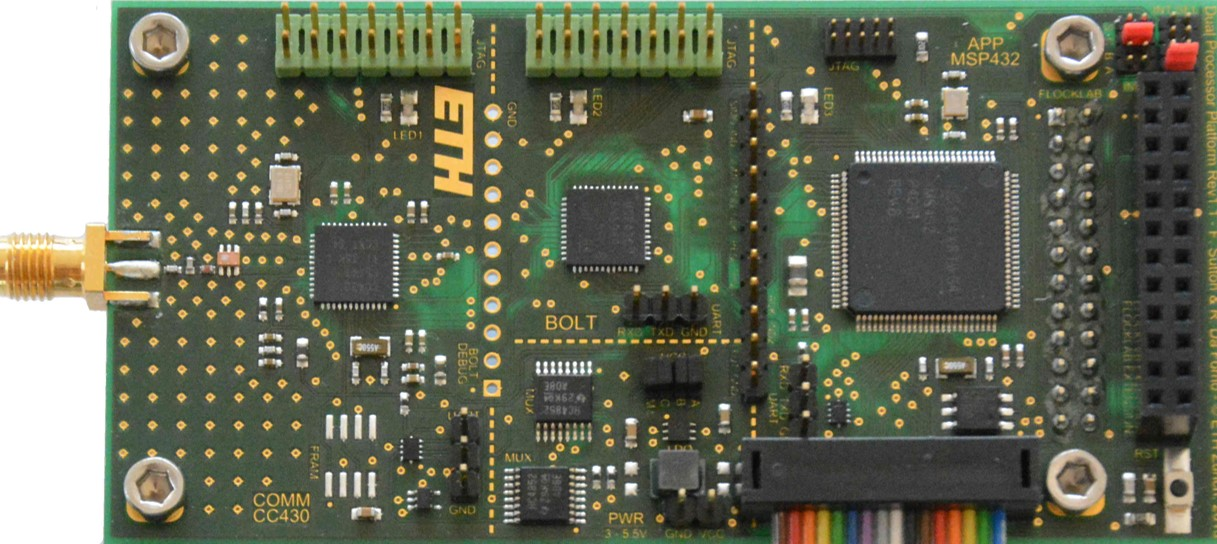
\includegraphics[width=0.8\linewidth]{DPPs/DPP-cc430}
	\caption{Integrated design of the same \DPP as in \cref{fig:dpp}, featuring a TI MSP432~\cite{msp432} as application processor (right) and a TI CC430 SoC~\cite{CC430F6137} as communication processor (left). \bolt sits in the middle, implemented on a TI MSP430 core featuring
64k FRAM~\cite{msp432FR}.}
	\label{fig:dpp-cc430}
\end{figure}

\begin{figure}[!b]
	\centering
	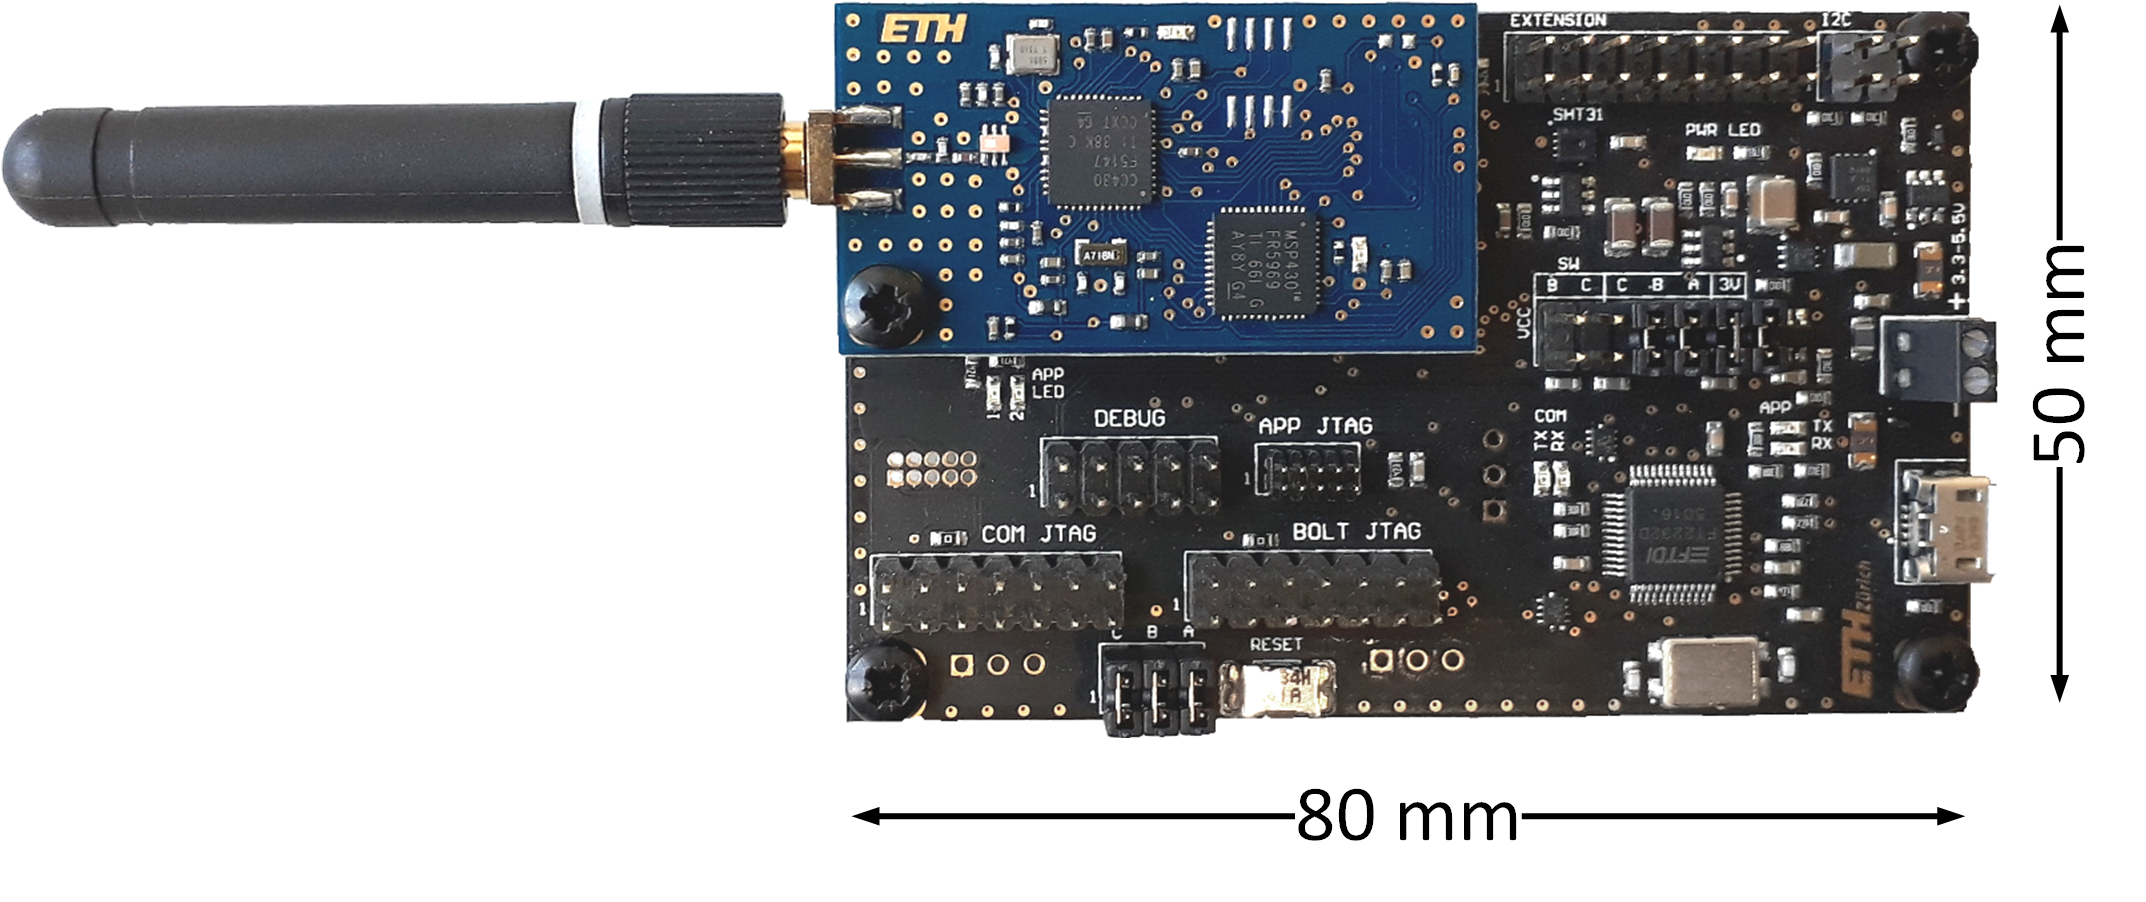
\includegraphics[width=\linewidth]{DPPs/DPP2-cc430}
	\caption{Redesign of the \DPP concept into two separated boards, called the \DPPtwo~\cite{beutel2019DPPdemo}. The lower board (black), called ``application development board'' hosts the application processor (in this case, a TI MSP432~\cite{msp432}) as well as all the I/O, power management, debugging, and other support functions. The upper board (blue) is called the ``communication board'' and hosts the communication processor (in this case, a TI CC430 SoC~\cite{CC430F6137}) and the \bolt interconnect.
	This platform has been used for a prototype wireless \CPS presented in \cite{mager2019Feedback, mager2019Demo} and discussed further in \cref{ch:ttw}.}
	\label{fig:dpp2-cc430}
\end{figure}

\begin{figure}
	\centering
	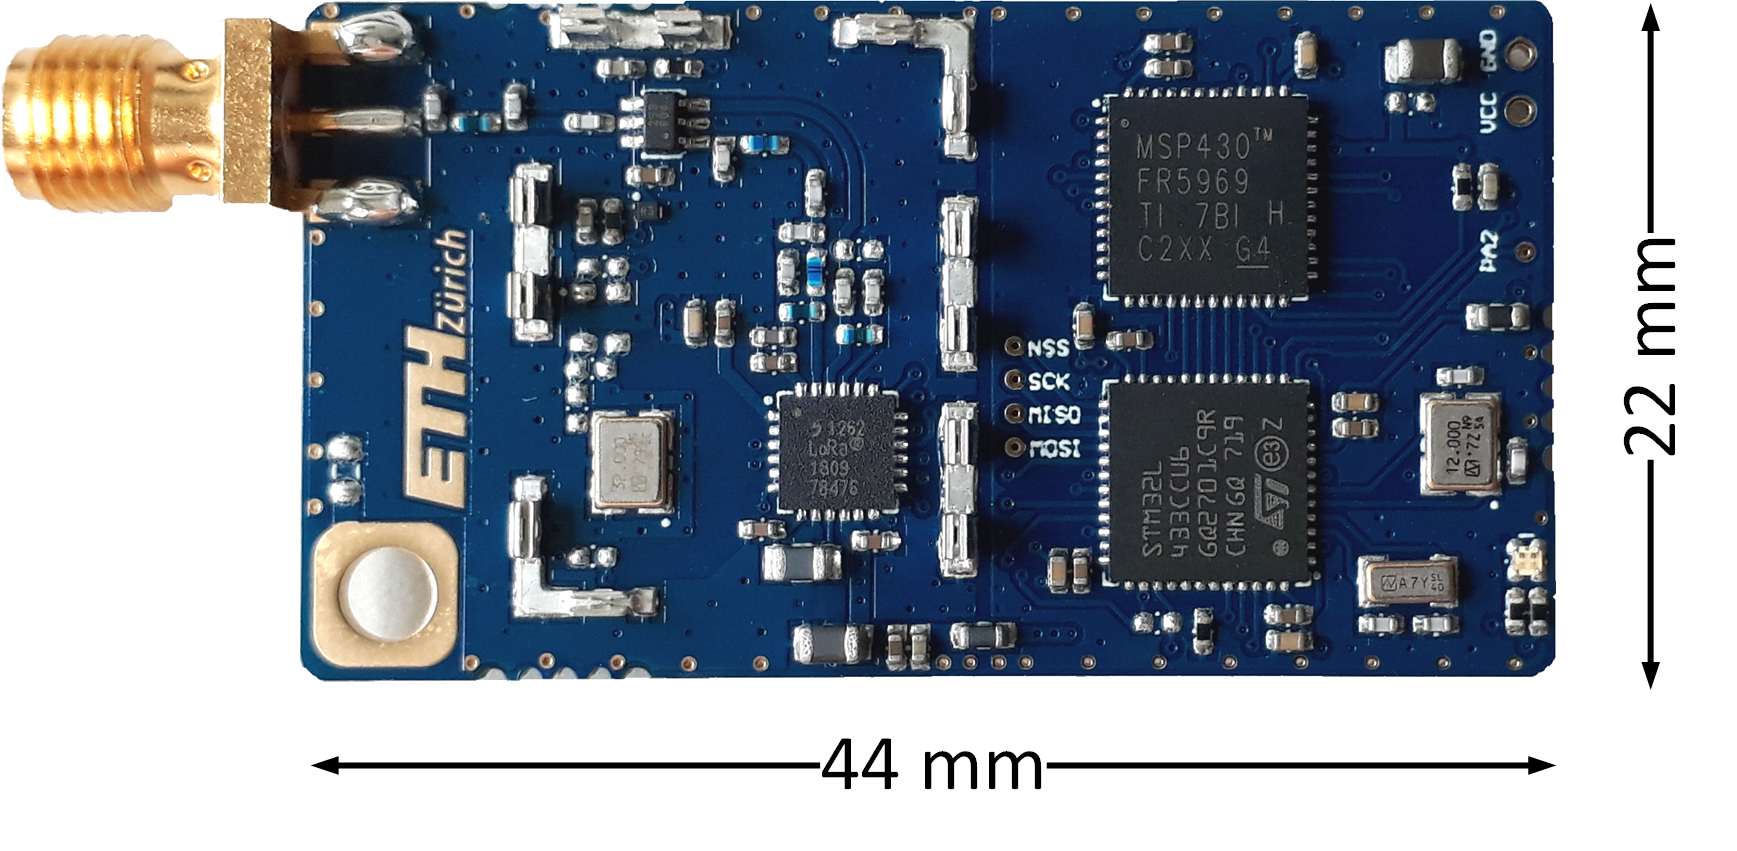
\includegraphics[width=0.8\linewidth]{DPPs/DPP2-LoRa}
	\caption{A different \DPPtwo ``communication board'' featuring a STM32L4 ARM core and Semtech latest generation long-range low-power LoRa transceiver with up to +22 dB m transmit power at 868 MHz (Semtech SX1262)~\cite{semtechSX1262}.}
	\label{fig:dpp2-lora}
\end{figure}

\begin{figure}
	\centering
	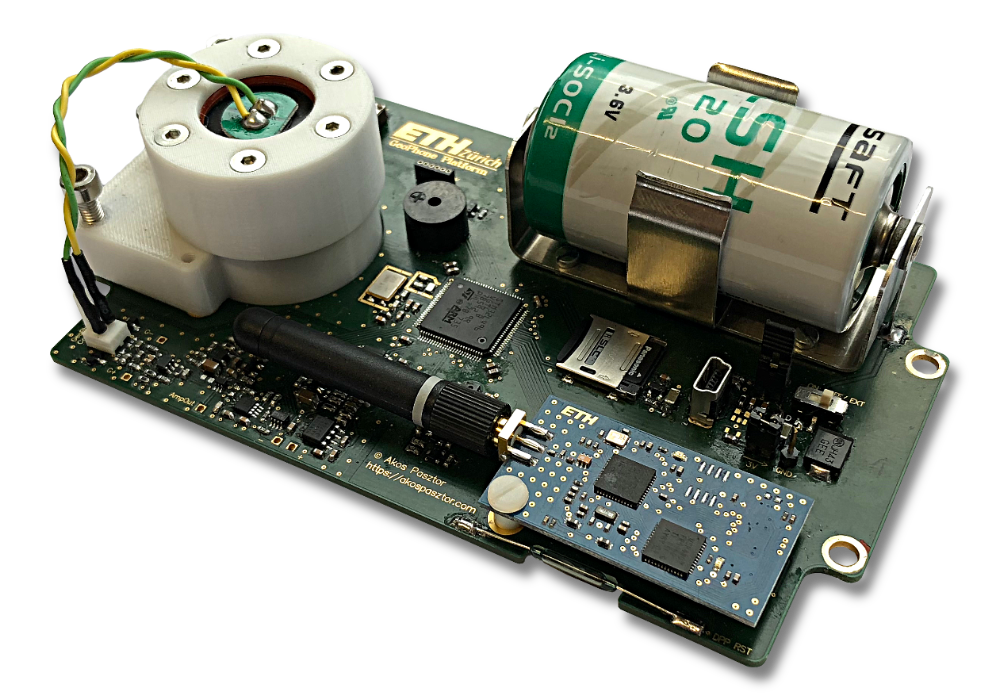
\includegraphics[width=\linewidth]{DPPs/GPP}
	\caption{Battery-powered geophone sensor node based on the \DPPtwo design.
	The lower ``application development board'' includes a geophone sensor, an analog low-power threshold-based wake-up circuit, and an ARM-Cortex M4~\cite{armCortexM4} as application processor.
	On top sits the same ``communication board'' as in \cref{fig:dpp2-cc430}.
	This design is currently deployed on the Hörnligrat of the Matterhorn~\cite{meyer2019IPSN}.}
	\label{fig:GPP}
\end{figure}

\end{subappendices}
